\section{Introduction}
\# \textbf{TODO introduzione da rifare, va ricentrata sullo scopo della tesi. Non so se ci vuole un'introduzione anche sul motion capture}
\\The human body is a marvel of complexity, 
seamlessly orchestrating an intricate symphony of movements 
that enable us to interact with the world around us. 
From the graceful ballet of a dancer to the powerful strides of an athlete, 
every motion we make is the result of a finely tuned interplay of physiological processes 
and biomechanical principles. 
Understanding the physical origins of movement is not only a fundamental pursuit 
in the fields of biology, physiology, and kinesiology, 
but it also holds the key to unlocking insights into human health, performance, and 
the very essence of our existence.

\subsection{Origins and technological rise of Motion Capture}
The roots of motion capture can be traced back to early attempts in the late 19th and early 20th centuries
to capture human movement for scientific analysis. 
These early endeavors laid the foundation for subsequent developments in the field. 
However, it wasn't until the latter half of the 20th century that motion capture 
began to gain traction as a viable technology.

From marker-based recording to detection through advanced sensors and high-definition cameras,
\begin{figure}[H]
    \centering
    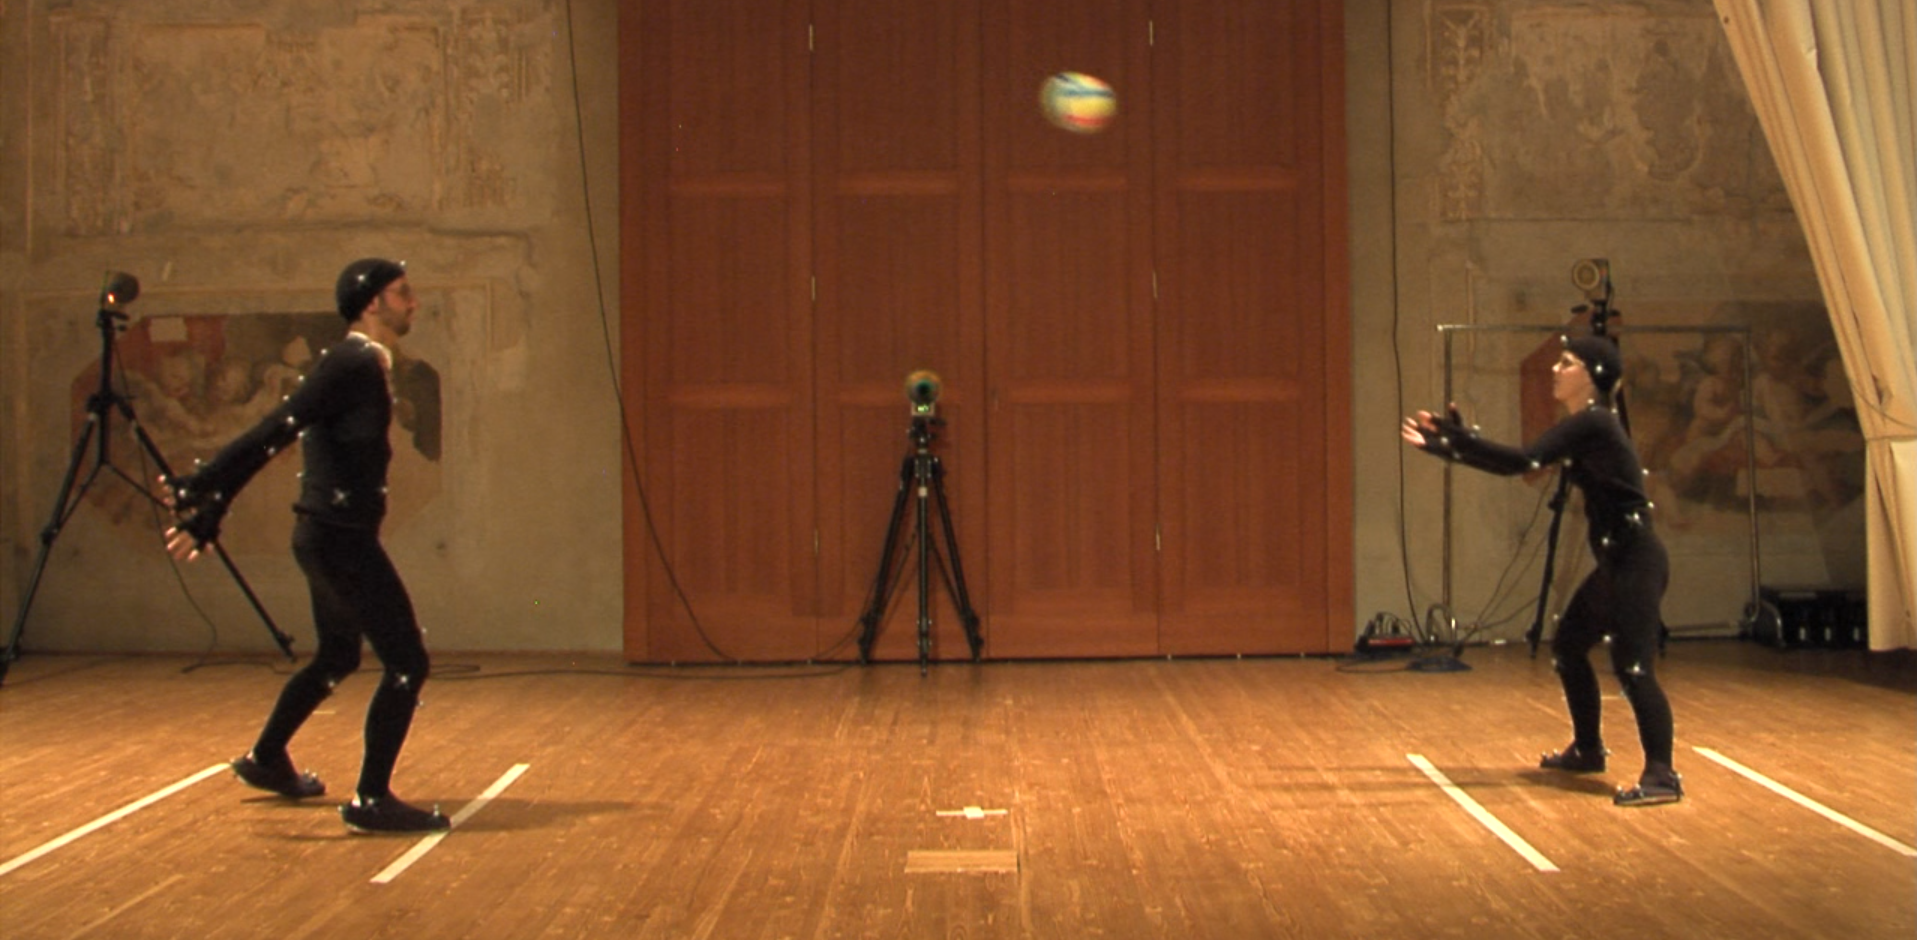
\includegraphics[width=0.9\textwidth]{graphics/bodyMarkersExampleImage.png}
    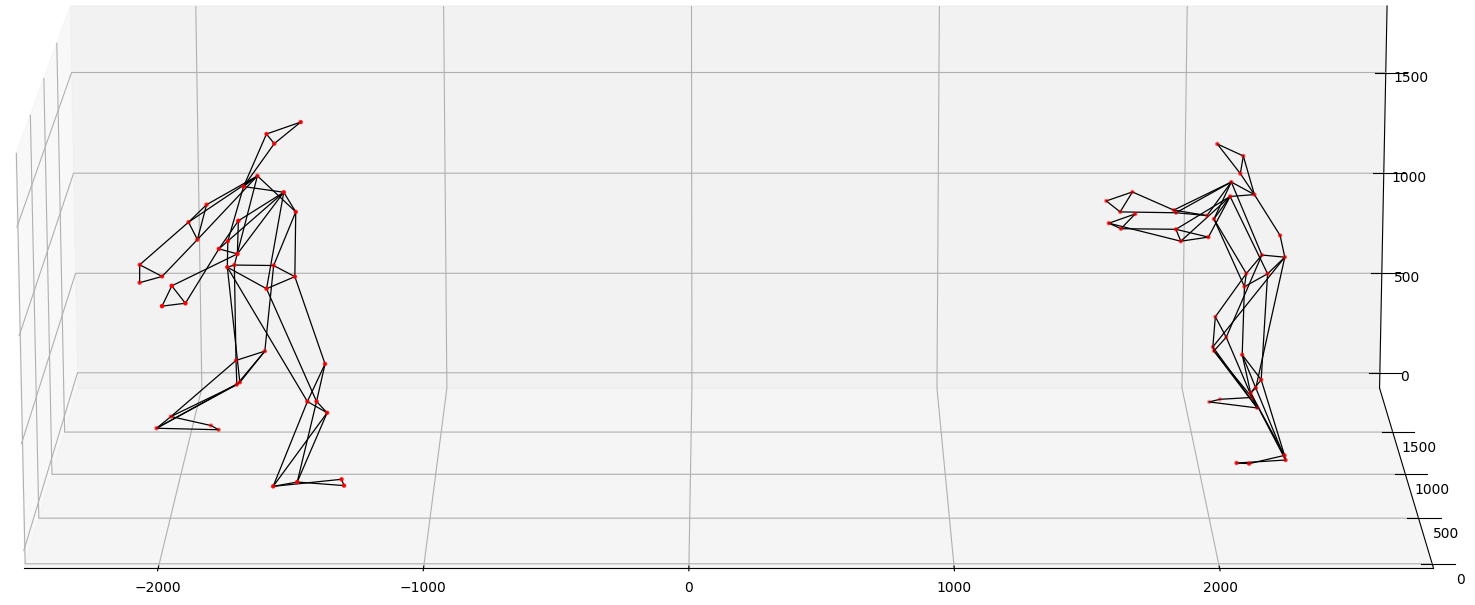
\includegraphics[width=0.9\textwidth]{graphics/bodyMarkersExampleMoCap.png}
    \caption{Video screenshot and MoCap scene with infrared cameras and markers}
    \label{fig:common}
\end{figure}

\begin{figure}[H]
    \centering
    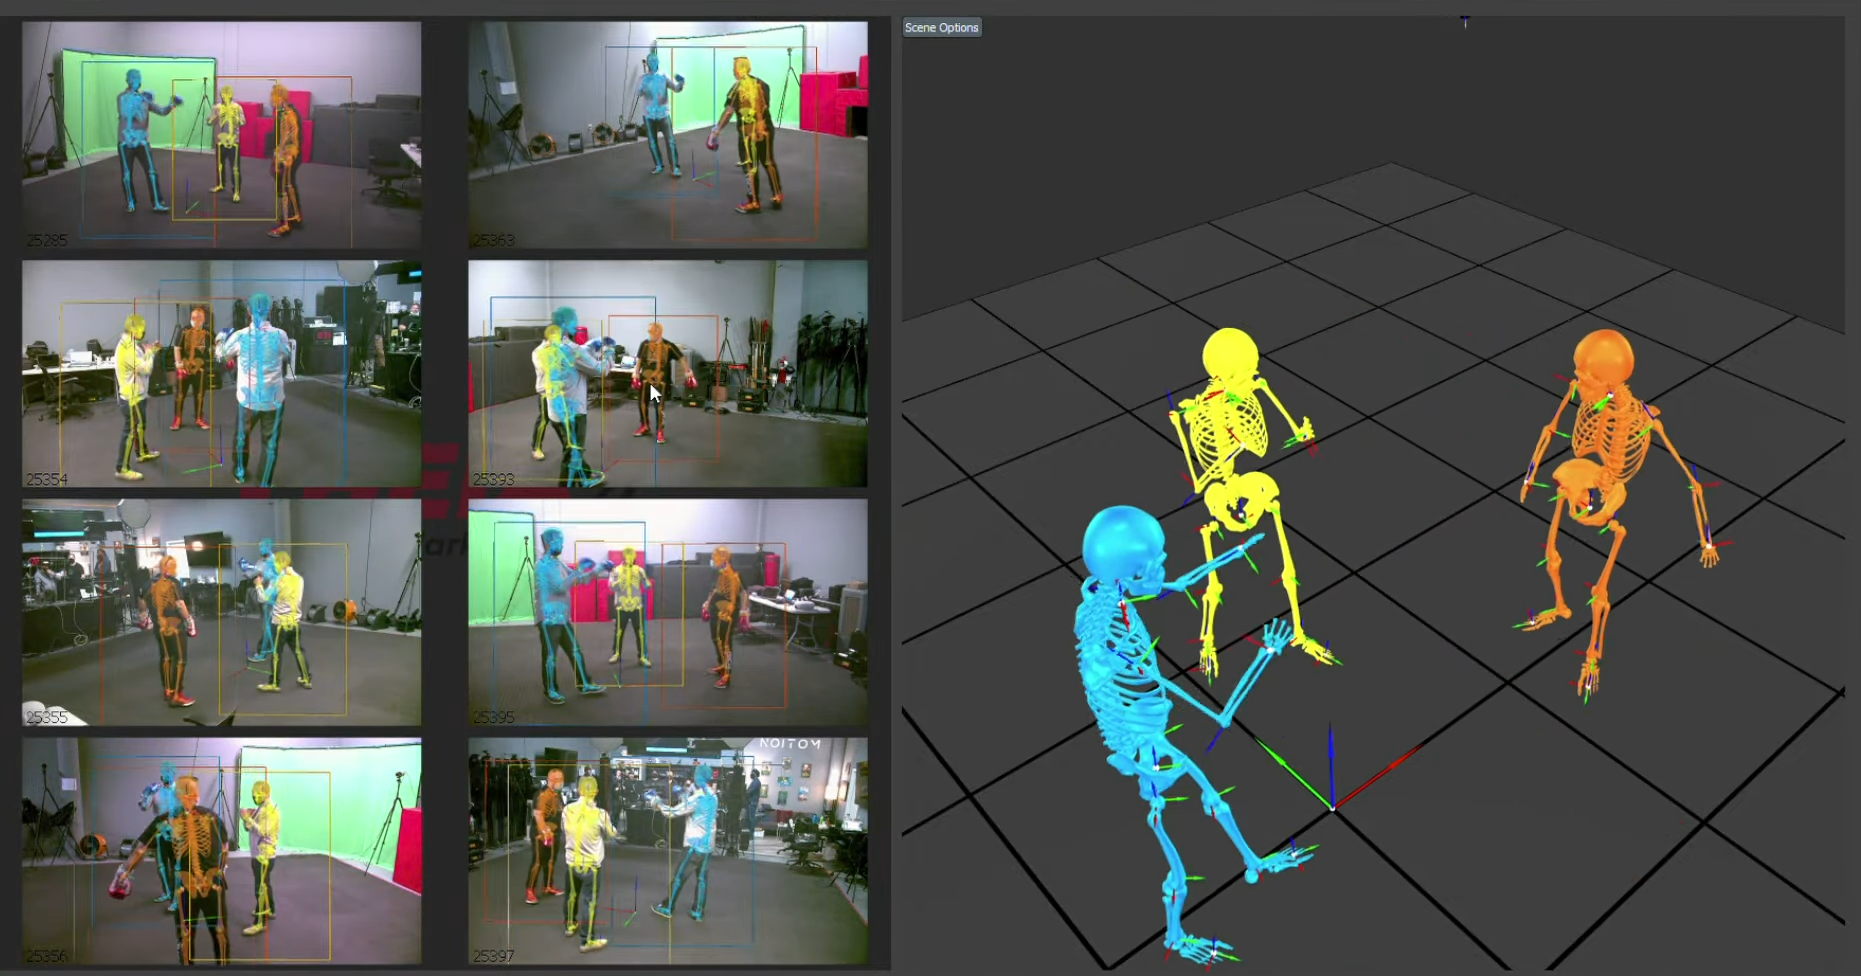
\includegraphics[width=0.9\textwidth]{graphics/MoCapMarkerlessQualisys.png}
    \caption{Markerless MoCap scene}
\end{figure}

we see how technological innovations have made the motion capture process increasingly precise and detailed.

\subsection{Research context}
Movement is one of the first complex actions that we learn when we are born. 
It defines how we interact with the world around us. 

Studies in this field date back to Charles Darwin in 19th century with his research in the relationship 
between movement and emotions, those that are called depressing do not lead to energetic actions. 
Pain, fear, and griefs when cause complete exhaustion results in prostration, 
while excitement of the nervous system is typically expressed through frenetic and vibrant movements \cite{darwin}.  

With the Laban Movement Analysis this field reached a formalization, applied to expressive motion in dance, 
in terms of what the body is doing, interrelationships within it, quality of the movement, 
changes in physical shape and harmonic interaction of the movement with the space around. 

In general, the analysis in full-body movement spaced both retroactively and proactively as form of expression to convey emotions. 
When moving our bodies, we are not simply performing a physical shift in space, but we use it also to 
communicate affective expressions to others in a nonverbal way \cite{gelder:2009,kleinsmith:2013,karg:2013}. 
For example, the behaviour behind a “caress” can vary from care to hostility, 
if the origin of that movement is either the wrist, the shoulder or if it involves a complex 
contraction of muscle torques from the arm down to the leg. 
This interconnection between many different body parts, brought us to the leading joint hypothesis \cite{dounskaia:2010} 
which offers a novel interpretation of control of human movements that involve multiple joints 
where the central nervous system organizes the execution of the motion act, with a hierarchical process 
that originates from a leading joint and propagates back to the body part that expresses the action. 
In sports and dance, the junction between effectiveness and efficiency of a movement, while also minimizing injuries on the long-term, 
lays in the awareness and exploitation of this concept. 
In my personal experience as a martial art athlete, understanding the correct motion, 
practicing and fixing misaligned posture is the key for an efficient energy allocation and the whole performance appearance. 
For example, the correct execution of a cross punch according to the common 
knowledge within the discipline consists of a complex 
twist of the upper body with a final braking involving hips, abdominal and back muscles, 
and the rear foot’s partial rotation \cite{wasik:2013}.
\begin{figure}[H]
    \centering
    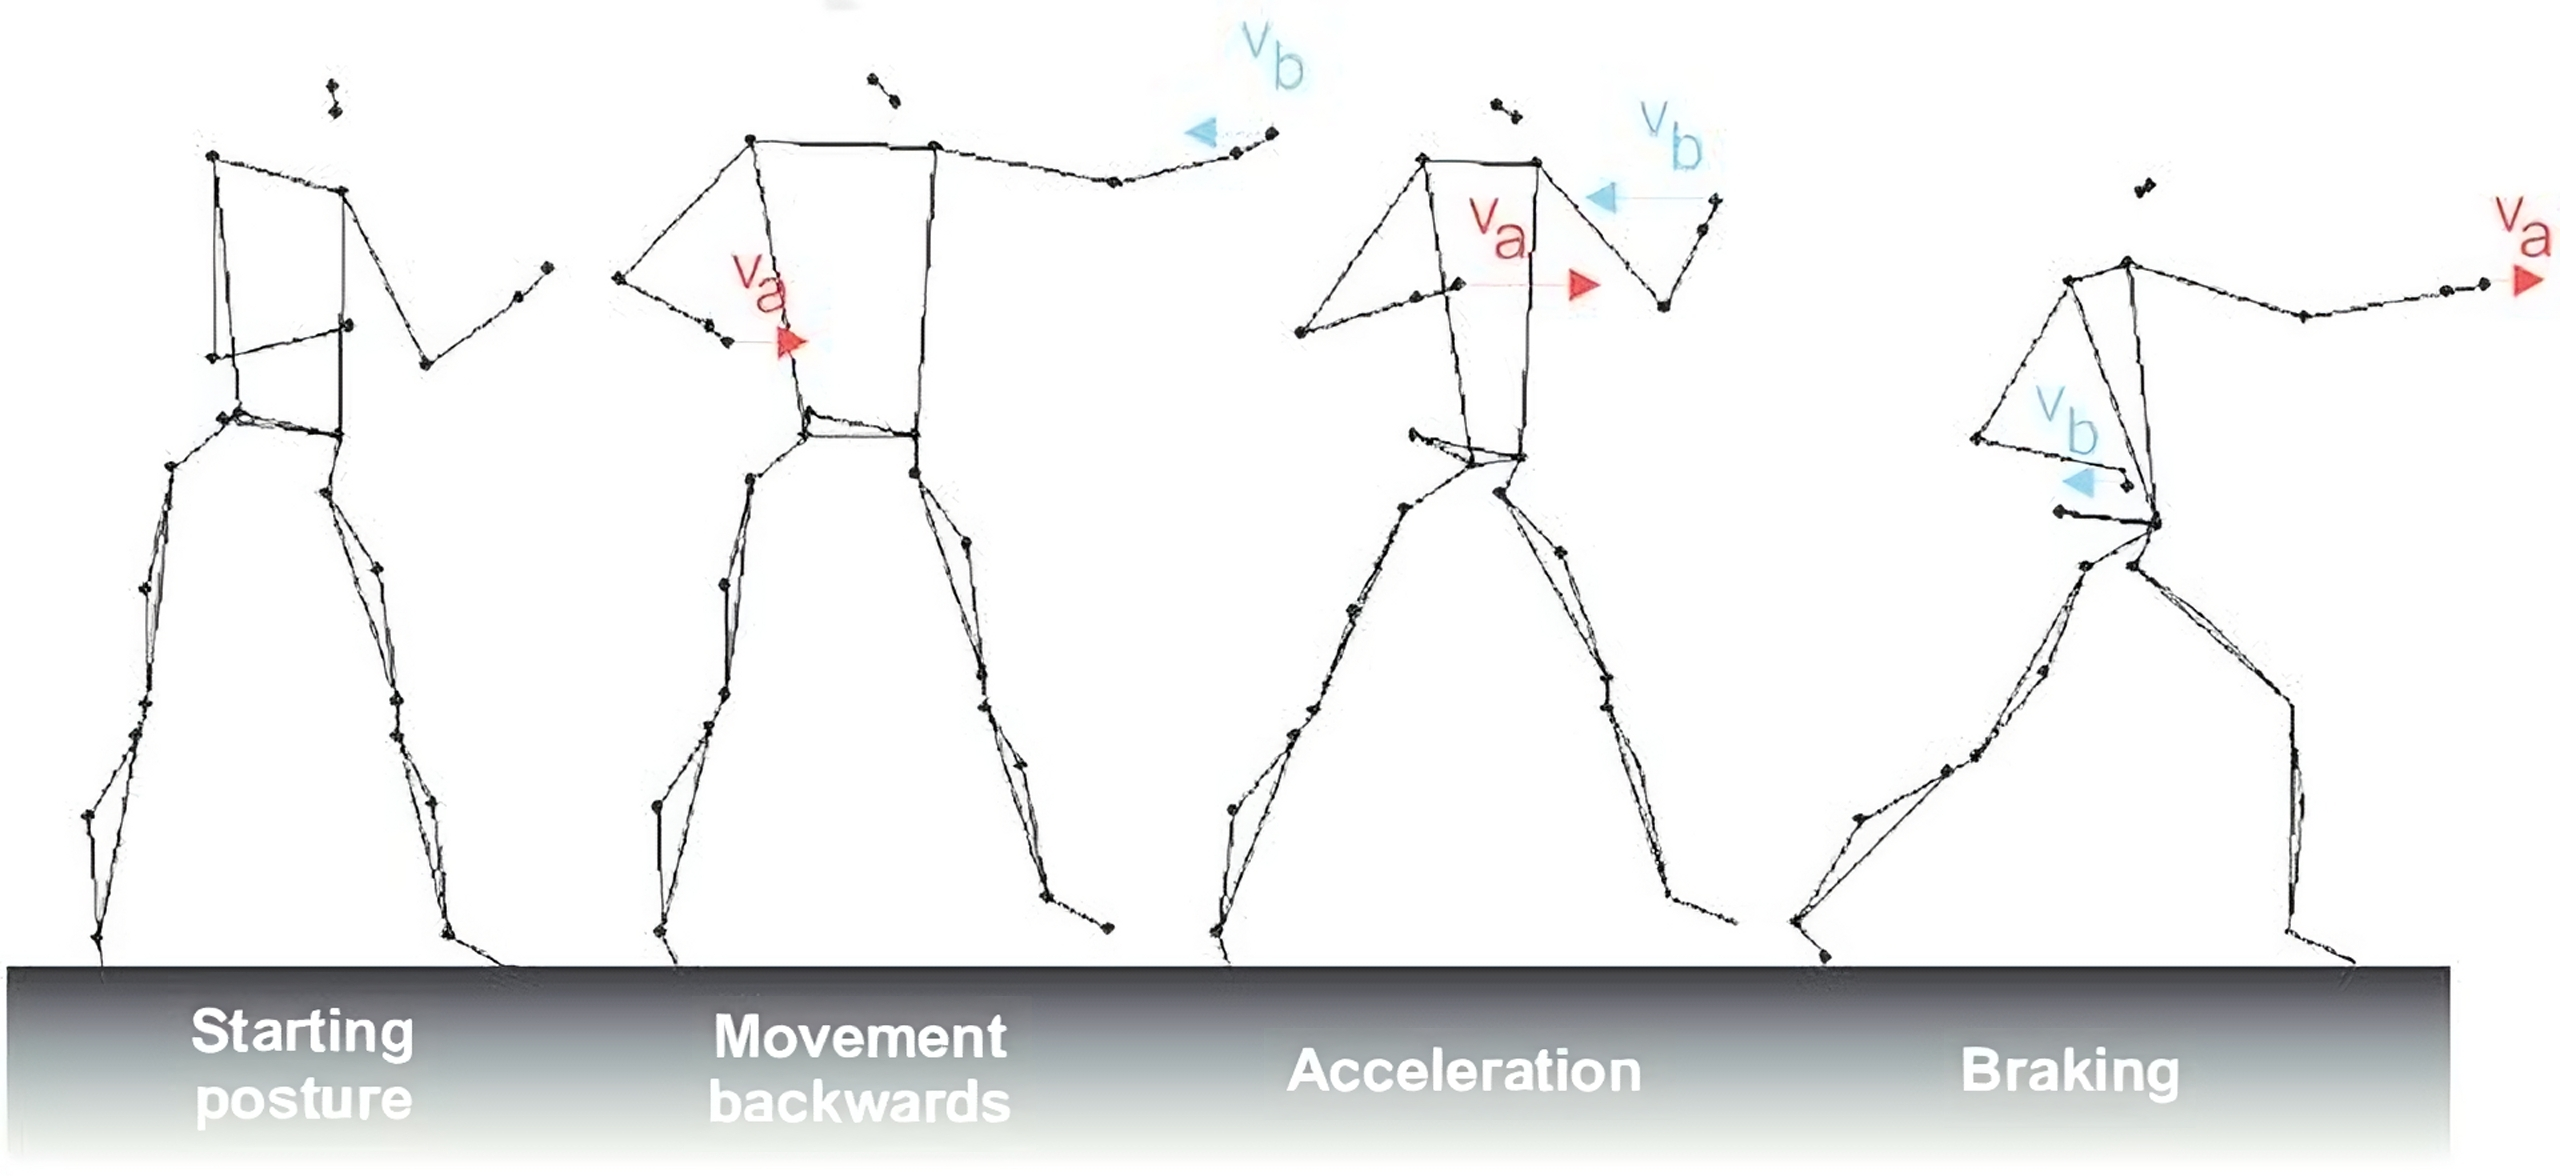
\includegraphics[width=0.9\textwidth]{graphics/Taekwon-do-joomuk-jirugi.jpeg}
    \caption{MoCap movement of the Taekwon-do joomuk jirugi}
    \label{fig:example}
\end{figure}